\subsection{Couches attention}

Le mécanisme d'attention est la partie centrale du transformeur qui réalise sa fonctionnalité.
Tous les autres modules sont une forme de prétraitement de son entrée ou de post-traitement de sa sortie. 
Chaque couche de l'encodeur implémente un module d'attention, 
tandis que chaque couche du décodeur en implémente deux.

Plusieurs types de mécanismes d'attention ont été proposés dans la littérature,
notamment l'attention additive \cite{Bahdanau_Cho_Bengio_2016} 
et l'attention multiplicative \cite{Luong_Pham_Manning_2015}.
Le transformeur utilise une variante de l'attention multiplicative appelée 
\foreignlanguage{english}{\emph{``scaled dot-product attention''}}~\cite{attention}.
Elle opère sur trois matrices \(Q, K, V\)%
\footnote{%
    De la terminologie anglophone : \foreignlanguage{english}{\emph{``Query'', ``Key'', ``Value''}},
    empruntée aux systèmes de recherche de l'information.
} de dimensions respectives \(d_Q \times l, d_K \times m, d_V \times n\),
qui représentent chacune l'encodage d'une séquence%
\footnote{
    \(d_Q, d_K, d_V\) sont les dimensions de plongement et \(l, m, n\) sont les longueurs des séquences.
    Notez que l'équation~\eqref{eq.scaled-dp-attention} impose les contraintes \(d_Q = d_K\) et \(m = n\),
    ce qui est vérifié pour les trois modules d'attention du transformeur.
}.
Le résultat est donné par l'équation~\eqref{eq.scaled-dp-attention}.
\begin{eqnarray}
    \label{eq.scaled-dp-attention}
    \text{Attention}(Q, K, V) = \text{softmax}\left(\frac{QK^T}{\sqrt{d_K}}\right)V 
\end{eqnarray}
Intuitivement, la \foreignlanguage{english}{scaled dot-product attention} peut être vue comme 
une forme de recherche floue dans une base de données.
Le terme \(QK^T\) est un produit scalaire entre les lignes de la requête \(Q\) et la clé \(K\).
Il représente la similarité entre les deux.
La fonction \(\text{softmax}\) le normalise pour obtenir des poids positifs de somme \(1\).
Enfin, le résultat et une somme des valeurs \(V\) pondérées par ces poids.
C'est dans ce sens-là qu'il s'agit d'une recherche floue :
les valeurs correspondantes aux clés qui répondent le mieux à la requête sont sélectionnées,
mais au lieu de renvoyer discrètement la meilleure valeur, 
toutes les valeurs contribuent dans la mesure de leur pertinence~\cite{CS480/680Lecture19_2019}.
La division par \(\sqrt{d_K}\) est une forme de régularisation. 
Elle permet d'éviter que le module de l'entrée du \(\text{softmax}\) devienne trop grand,
ce qui rend son gradient trop petit ainsi ralentissant l'apprentissage%
\footnote{%
    Le choix de la valeur de \(\sqrt{d_K}\) n'est pas arbitraire.
    Sous l'hypothèse que les valeurs de \(Q\) et \(K\) sont centrées et réduites,
    les valeurs de \(QK^T\) sont centrées de variance \(d_K\).
    La division par \(\sqrt{d_K}\) les ramène à une variance de \(1\)~\cite{attention}.
}~\cite{attention}.

\begin{figure}[hbt]
    \centering
    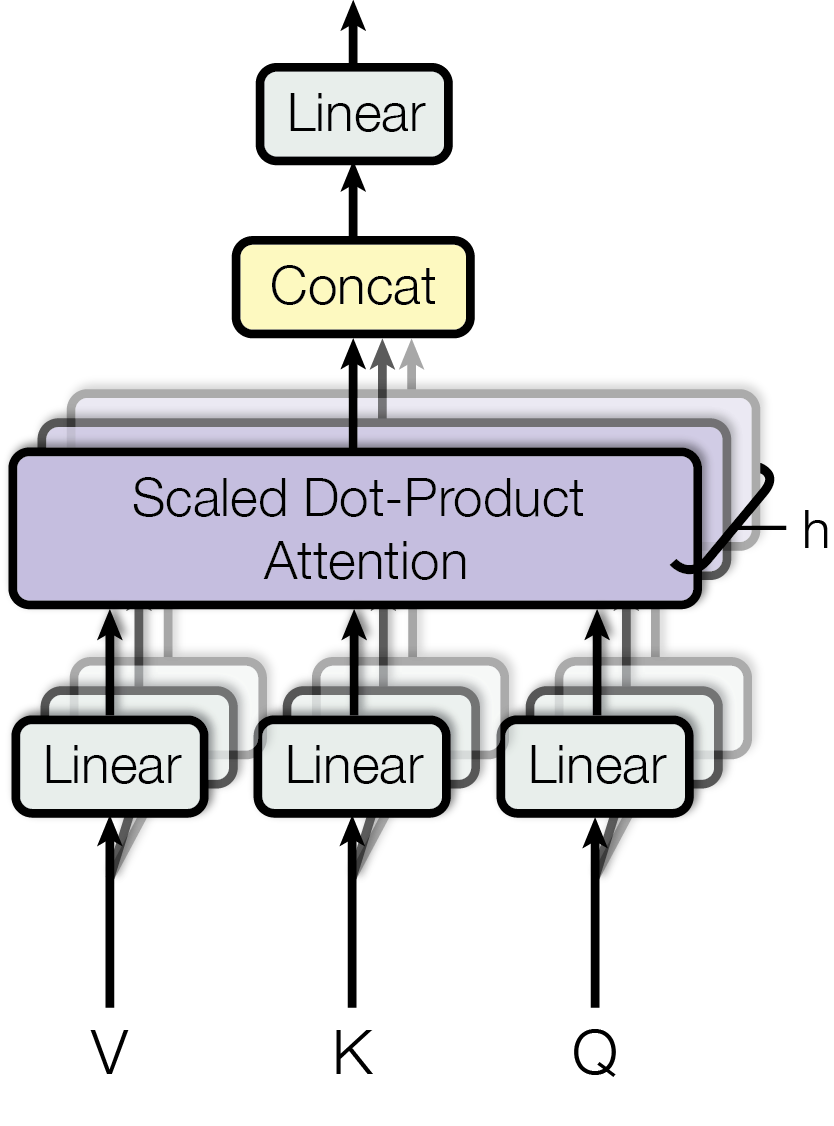
\includegraphics[height=5cm]{assets/images/multihead-attention.png}
    \caption[Schéma d'une couche attention multitête.]
    {Schéma d'une couche attention multi-tête~\cite[Fig 2]{attention}.}
    \label{fig.multihead-attention}
\end{figure}

Les auteurs de~\cite{attention} ont observé une amélioration de la performance 
en utilisant plusieurs modules (ou têtes) de \foreignlanguage{english}{scaled dot-product attention},
projetant les entrées différemment avant de les passer à chaque tête.
Les sorties des têtes sont concaténées et passées à une couche linéaire qui produit la sortie finale.
Les projections sont réalisées par des couches linéaires entraînables et le nombre \(h\) de têtes est un hyperparamètre fixé à \(8\) par les auteurs%
(Voire la Figure~\ref{fig.multihead-attention}).

\subsection{Auto-attention et attention croisée}

La couche attention de l'encodeur et la première couche attention du décodeur sont des couches
d'\emph{auto-attention} i.e leurs requêtes, clés et valeurs sont les mêmes.
L'auto-attention du décodeur se distingue de celle de l'encodeur par la présence du \emph{masque}.
En produisant un élément de la séquence de sortie, le décodeur ne doit faire attention qu'aux éléments
qui le précèdent.
Toutes les autres valeurs doivent avoir un poids nul.
Pour ce faire, la matrice \(M\) 
\begin{equation}
    M_{ij} = \begin{cases}
        0 & \text{si } j > i \\
        -\infty & \text{sinon}
    \end{cases} 
    = \begin{bmatrix}
        -\infty & -\infty & \cdots & -\infty \\
        0       & -\infty & \cdots & -\infty \\
        \vdots  & \vdots  & \ddots & \vdots \\
        0       & 0       & \cdots & -\infty
    \end{bmatrix}
\end{equation}
est ajoutée à l'entrée de la fonction \(\text{softmax}\).

La deuxième couche attention du décodeur est une couche d'\emph{attention croisée}.
Les requêtes viennent de la sortie et les clés et valeurs viennent de l'entrée.
Cette couche calcul les dépendances entre l'entrée et la sortie,
tandis que les deux autres couches calculent les dépendances à l'intérieur de l'entrée et de la sortie.
C'est cette couche qui permet au décodeur de conditionner sa sortie sur l'entrée.


